\chapter{Designing an approach}
In this chapter I lay out the design goals, the main design and the decisions which led to them.


\section{Defining system boundaries}
\subsection{Thread model}
As an \defref{adverser} we assume the following attributes:
\begin{itemize}
\item Available founding is huge.
\item Can have own mailer infrastructure.
\item Is able to read, write or modify network data freely at any point of the net.
\end{itemize}
His intensions are:
\begin{itemize}
\item Discover message flows
\item Discover message contents
\item Identify users of the system
\end{itemize}

\subsection{User model}
The assumed \defref{user} of the system is:
\begin{itemize}
\item Does care about privacy.
\item Does or does not have support from a mail server admin.
\item Has no special computer knowhow.
\item Has the ability to install a program or plugin on his personal computer.
\item Has no cryptographic knowhow.
\item Is using a device with enough calculation power to solve cryptographic tasks.
\end{itemize}

His intensions are:
\begin{itemize}
\item Send personal or confidential Information securely to another user
\end{itemize}
His expectations are:
\begin{itemize}
\item System should be easy to configure and maintain (in an ideal world: Zero touch). 
\item System should be fast.
\item System should be reliable.
\item System should work on any client he is using.
\item System should not be a legal problem to him or any of his peers.
\end{itemize}

\subsection{Mail server admin model}
The assumed \defref{mail server admin} of the system is:
\begin{itemize}
\item Does care about privacy.
\item Has considerable computer knowhow.
\item Has the ability to install a program or plugin.
\item Has possibly no cryptographic knowhow.
\item Does know his own mail infrastructure.
\item Is using a device with enough calculation power to solve cryptographic tasks.
\end{itemize}
His intensions are:
\begin{itemize}
\item Support his users in sending personal or confidential information securely to another user
\end{itemize}
His expectations are:
\begin{itemize}
\item System should be easy to configure and maintain (in an ideal world: Zero touch). 
\item System should be fast.
\item System should be reliable.
\item System should work on any client he is using.
\item System should not be a legal problem for him or his company.
\item System should still allow him to do regulatory tasks such as virus scanning or backup.
\end{itemize}

\section{Basic Requirements of an Approach}
Different types of peers must be available:
\begin{itemize}
  \item Passive\\
	This peer is sending and receiving only. It works as a endpoint for communication and does only allow relay transfer for messages containing payload for this peer.
	\item Stealth\\
	This peer is behaving absolutely passive to unknown peers. No automatic replys are beeing sent unless the sender has been identified. Sender identification may be based on any criteria such as SMTP AUTH, known identity to vortex or knowledge about the public key of the recipient.
	\item public\\
	This peer is publicly known to be a participating peer. It may be used for local or relay delivery.
\end{itemize}

\subsection{Transport Layer Blending}
In order to blend into SMTP-Transport layer the following Criterias should be met:\par
\begin{table}[H]
  \centering
	\def\fh{\multicolumn{1}{|l}{\textbf{Criteria}} &
	\multicolumn{1}{|l}{\textbf{Parameter}} &
	\multicolumn{1}{|l|}{\textbf{Reason}}}
	\tablefirsthead{\hline\fh\\\hline}
	\tablehead{\hline\multicolumn{3}{|l|}{\small\slshape continued from previous page}\\\hline\fh\\\hline}
	\tabletail{\hline\multicolumn{3}{|l|}{\small\slshape continued on next page}\\\hline}
	\tablelasttail{}
	\bottomcaption{Transport layer decisions}
  \begin{supertabular}{|>{\raggedright\arraybackslash}p{3cm}|>{\raggedright\arraybackslash}p{3cm}|>{\raggedright\arraybackslash}p{6cm}|}
		SMTP address & May have non mandatory extensions & SMTP adresses may have extension. However, these extensions must not be mandatory since a target address must be able to be in stealth mode\\\hline
		Transfer channel negotiation & Should always use SMTPS or STARTTLS & Hide immediate peer partners. This increases amount of work to be done for analyzing traffic.\\\hline
		encoding mime message & Should always use Base64 & Any other encoding would differentiate MailVotex from regular traffic\\\hline
		Transport media & Attachment & May be any kind of attachment. Recommended are mime types which have no verifiable structures such as .raw or .pcm files to avoid detection thru content analysis.\\\hline
	\end{supertabular}
\end{table}
FIXME incomplete section

\chapter{Specifying a target solution}
\section{General}
We have chosen a general message approach which may use any established message passing protocol as a carrier. In general we use an existing protocol (or protocol set) as carrier to transport the message (transport layer) on top of this layer we have a layer handling all presentation concerns for the transport layer (shaping layer). This layer handles the building of the message (including but not limited to steganographic messages and dead parrot avoidance). The Topmost layer handles all messages, calculates next hops and queues messages (routing layer). It takes furthermore care of the error handling.\par

The routing layer has a couple of partnering blocks. The main Block is called ``router''. 

The next important block is the accounting helper. This building block takes care of all states required to manage the system . It stores identities and quotas and authorizes messages to be routed. 

The integrity helper collects messages authenticates and checks the integrity. It gets messages from the inbound queue

The queue helper maintains queues of the system. 

\subsection{Application Design}
We first have to define the main hook for our solution. While most of the sent messages are always passed from server to server using SMTP the protocols for accessing a mailbox are varying. The most common interfaces within the private mail traffic are \defref{POP} and \defref{IMAP}. In the business environment it is mainly \defref{IMAP} or \defref{MS-OXMAPIHTTP}. \par

I will use \defref{IMAP} as my hook to the mail account to maximize portability. The Solution is based on a \defref{IMAP} proxy server able to join encrypted delivered data with ordinary data. This hook provides means to turn any mailbox into a vortex\par

Final goal should be let the device run on a RASPI-Device (or similar) with permanent internet access. \par

For message sending I will implement an SMTP relay server. This relay server only accepts authenticated messages. The messages shall be scanned for header requesting a specific type of security. The message then is packaged according to these specs and forwarded to the outgoing SMTP server.

All operation carried out on mails are implemented in a thread safe library called libVortex. The API should be stable and suitable for thirdparty apps to be used. Around this a series of connectors are implemented.

\begin{figure}[H]
  \centering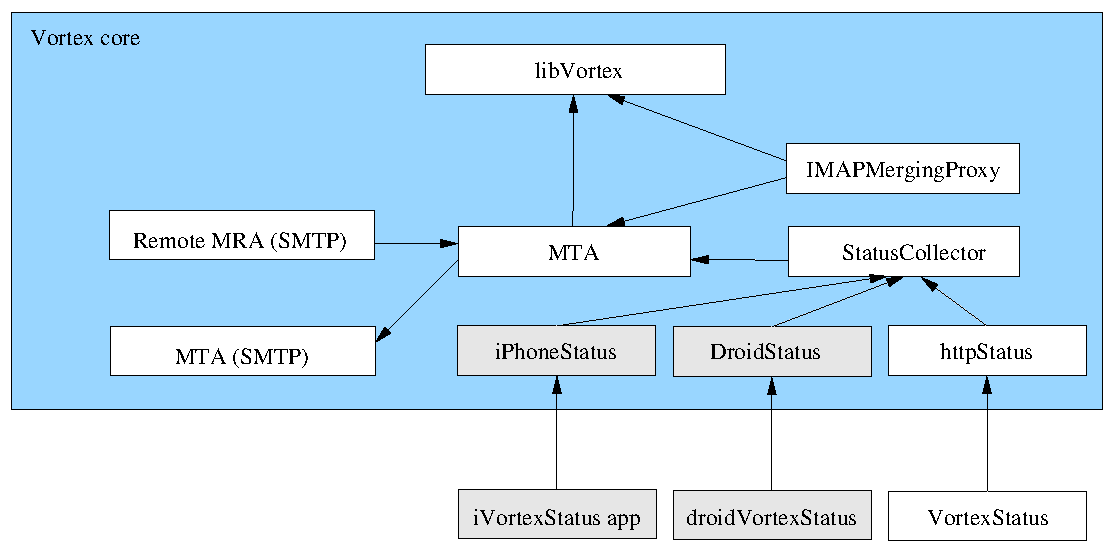
\includegraphics[width=\textwidth]{inc/VortexModules}
  \caption{Vortex Modules}\label{fig:VortexModules}
\end{figure}

Main language of the core will be Java for portability reasons. All GUI relevant parts are not part of the core to improve portability.\par

Platform specific status apps are not created as part of this work. They are however built in a way so that they may

\subsection{Third Party Code}
\subsubsection{Java}
The code will be written in Java 7 compliant code. And allThe JDK beeing used is OpenJDK (\url{http://openjdk.java.net/}). As a crosscompiler I do use gcj (\url{http://gcc.gnu.org/java/}). All configuration is either done in files or using a http interface.

\subsubsection{SQL Server}
As the main local database backend H2 is used. 

\subsubsection{Mail Server}
Base for all local caching and intermediate mail services a Hedwig Mail Server will be used. However This code will undergo heavy modifications.

\subsection{Folder storage}
The configuration data is stored in a IMAP folder. To hide the IMAP store to an observer the client is provided with a folder name and password (instead of a fixed folder name). The key for all config data and all messages is stored in a message in this folder. The folder is hidden by the proxy if known.

\subsection{Protocol Design}
\subsubsection{General Design}
The protocol is based on serveral Design criterias. It is important to understand that the protocol does not trust any infrastructure exept the own. It is therefore based on a zero trust infrastructure. It splits up into the layers transport, obfuscation and routing. Whereas routing may be split up in accounting, queuing.

\begin{figure}[H]
	\centering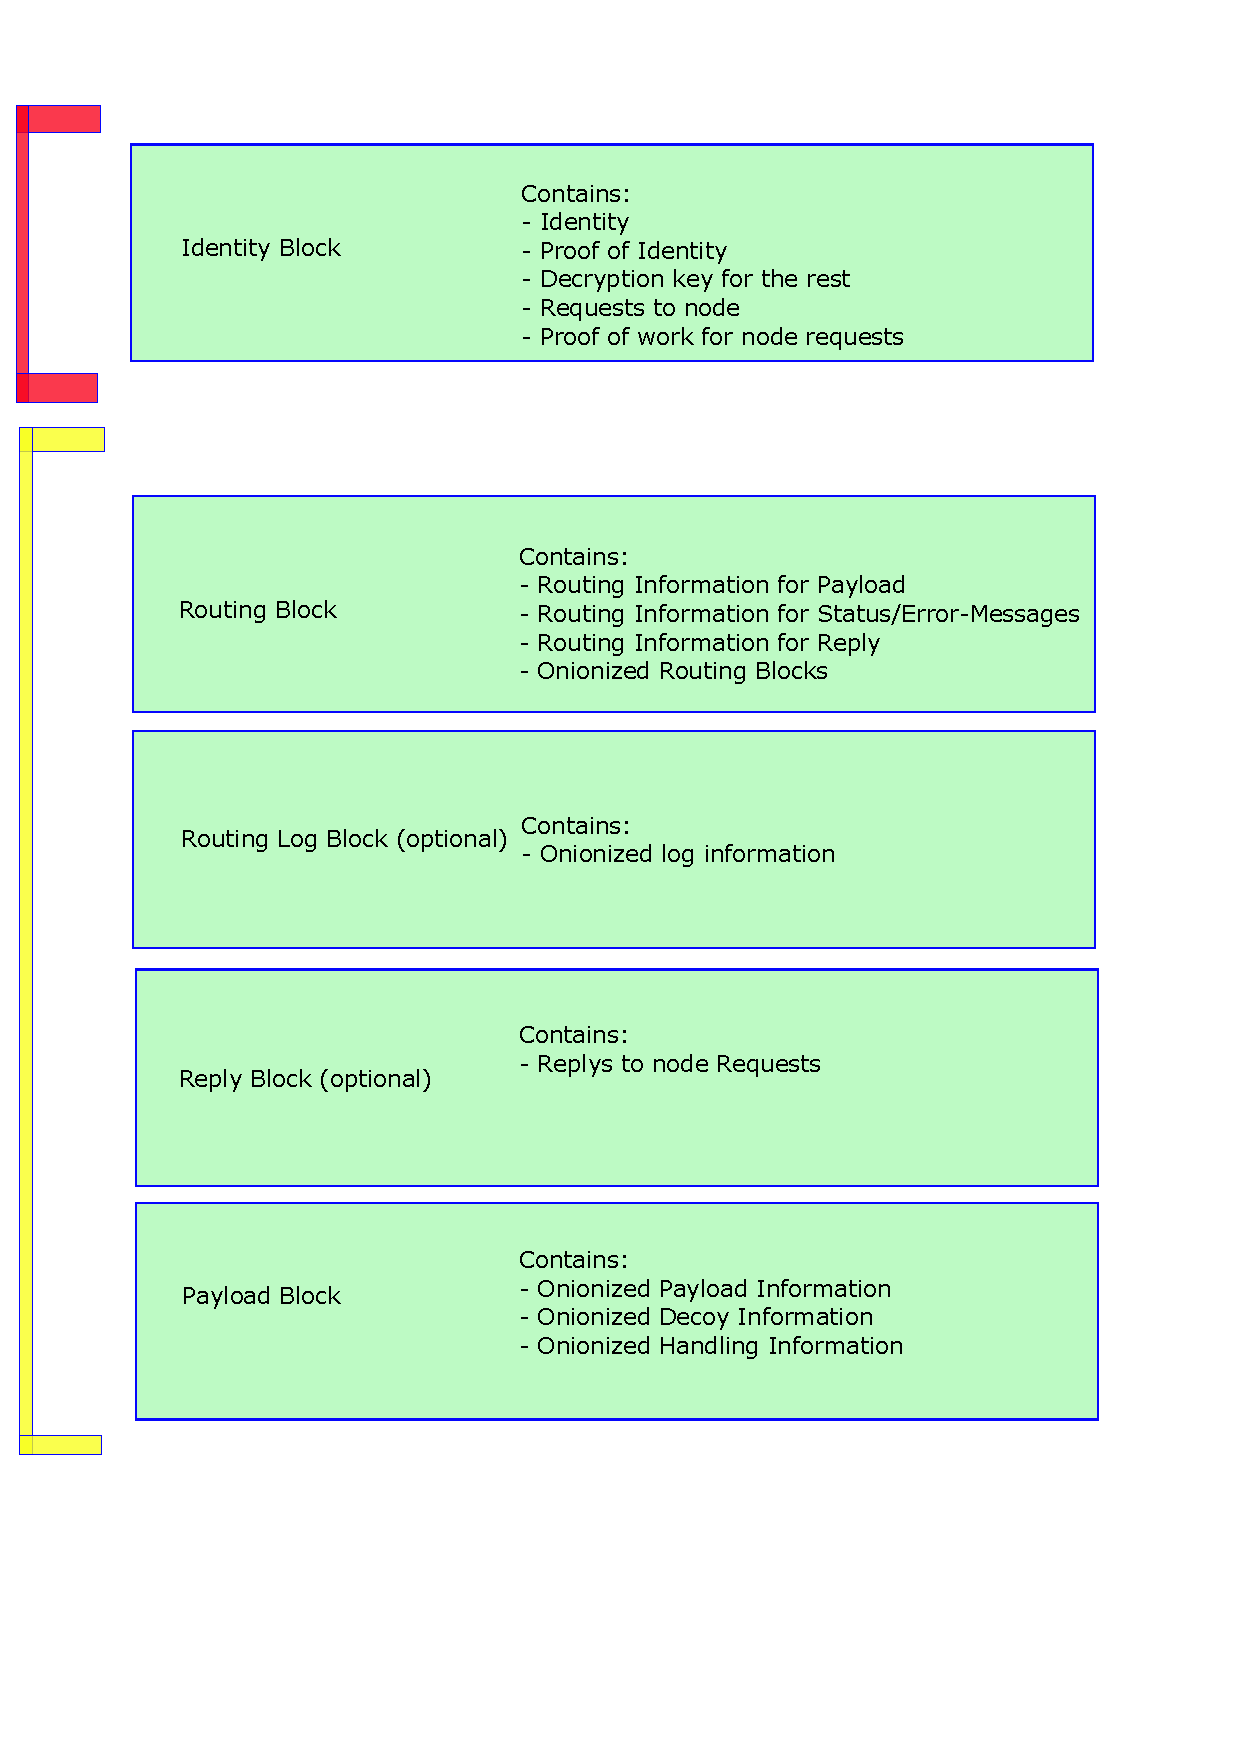
\includegraphics[width=0.6\textwidth]{inc/parts/PrinciplesOfProtocol.pdf}
	\caption{Vortex Modules}\label{fig:PrinciplesOfProtocol}
\end{figure}


\subsubsection{General Process of Communication}
FIXME incomplete section

\subsubsection{General Process of Bootstrapping}
FIXME incomplete section

\subsubsection{General Information about Encryption and Hashing\label{sec:genEncrypt}}
In This Protocol a lot of encryption and hashing algorithms have been chosen. This Choice should be explained. 

First of all we need a subset of encryption algorithms all implementations may rely on. Defining such a subset garatees interoperability between all nodes regardless of their origins. 

Secondly we need to have a spectrum of algorithm in such a manor that it may be (a) enlarged if necesary and (b) there is an alternative if an algorithm is broken (so that algorithms may be withdrawn if required without affecting the function in general). 

And third due to the onion like design described in this document asymetric encryption should be avoided in favour of symetric encryption to minimize losses due to the key length and the generally higher CPU load oposed by asymetric keys.

If the algorithm is generally bound to specific keysizes (due to S-Boxes or similar constructs) the key size is incorporated into the definition. If not the key size is handled as parameter.

The keysizes have been chosen in such a manor that the keytypes form tupples of approximately equal strength. The support of Camelia192 and Aes192 has been defined as optional. But as they are wildly common in implementations they have allready been standardized as they  build a possibility to step up security in future.

Having this criterias for choice I chose to use th following keys and keysizes:
\begin{itemize}
	\item Symetric
	\begin{itemize}
		\item AES (Keysizes 128, 192, 256)
		\item Camellia (Keysizes 128, 192, 256)
	\end{itemize}
	\item Asymetric
	\begin{itemize}
		\item RSA (Keysizes free)
		\item DSA
		\item Named Elliptic Courves
		\begin{itemize}
			\item secp384r1
			\item sect409k1
			\item secp521r1
		\end{itemize}
	\end{itemize}
	\item Hashing
	\begin{itemize}
		\item sha384
		\item sha512
		\item tiger192
	\end{itemize}
\end{itemize}



\subsection{Block Details}
\subsubsection{Preamble}
The following sections contains exact building information about the blocks used by the Protocol. It contains handling instructions and validity ranges.
FIXME incomplete section

\subsubsection{Routing block}
FIXME incomplete section

\subsubsection{Address request block}
FIXME incomplete section

\subsection{Messages}
FIXME incomplete section

\subsubsection{Basecom}
FIXME incomplete section

\section{libVortex}